\documentclass[11pt,a4paper]{article}
\usepackage[margin=2.2cm]{geometry}
\usepackage[T1]{fontenc}\usepackage{lmodern}
\usepackage{graphicx,booktabs,amsmath,siunitx,hyperref,listings,xcolor}
\hypersetup{colorlinks=true,linkcolor=blue!50!black,urlcolor=blue!50!black,citecolor=blue!50!black}
\lstset{basicstyle=\ttfamily\footnotesize,backgroundcolor=\color{gray!8},frame=single,breaklines=true}

\title{Adsorption of Mercury on Gold Surfaces with Machine-Learned Interatomic Potentials in ASE}
\author{Aszad [Surname]\\[2pt]\small Project report for the INTEREST programme, JINR Dubna (project 411, proposed by Prof.\ M.\ Ilia\v{s})}
\date{\today}

\begin{document}
\sloppy
\maketitle

\begin{abstract}
Mercury is the lighter homolog of copernicium (Cn, $Z=112$), whose chemistry is probed by single-atom
thermochromatography on gold-covered detectors. Following the project plan, I set up a Linux (WSL2/Ubuntu)
environment, ran the baseline ASE scripts of the \texttt{open-collection} repository, and extended them into a
production workflow that computes Hg adsorption energies on all high-symmetry sites of Au(111), Au(100) and
Au(110) with two universal machine-learned interatomic potentials (MLIPs), MACE-MP-0 and CHGNet. Both models
agree on the physics: Hg prefers hollow sites, binding strengthens with the number of Au neighbours, and the
open facets bind more strongly than the close-packed Au(111). Quantitatively they differ by
9--23\,kJ/mol; CHGNet ($-91.5$ to $-113.7$\,kJ/mol at the best sites) is closer to the experimental
$-\Delta H_\mathrm{ads}\approx\SI{98}{kJ/mol}$ than MACE-MP-0 ($-74.7$ to $-92.2$\,kJ/mol). I also show that the
baseline set-up (lattice constant fixed to \SI{4.08}{\AA}, one site) underestimates binding by
about \SI{5}{kJ/mol}, and that the results are converged to $\approx\SI{1}{kJ/mol}$ with respect to slab
thickness, cell size and vacuum.
\end{abstract}

\section{Introduction}
The chemical characterisation of superheavy elements relies on gas-phase thermochromatography, where single
atoms deposit on a temperature gradient of gold-covered detectors; the deposition temperature is translated
into an adsorption enthalpy. For Cn, Eichler \emph{et al.}\ measured $-\Delta H_\mathrm{ads}(\text{Au})
=52^{+4}_{-3}$\,kJ/mol~\cite{eichler2007}, much weaker than for its homolog Hg ($\approx98$\,kJ/mol~\cite{eichler2013}).
Atomistic modelling of the Hg/Au system is therefore the natural benchmark before any calculation on Cn.
Density functional theory is the standard tool, but it is costly for the many sites, facets and set-ups that
need to be compared. Universal MLIPs promise near-DFT accuracy at a fraction of the cost. The goal of this
project is to test how far such potentials can be trusted for Hg on gold, using the Atomic Simulation
Environment (ASE)~\cite{ase}.

\section{Computational environment}
All work was done on a Windows laptop in a WSL2 Ubuntu terminal. A Python virtual environment
(\texttt{ase-env}) holds ASE, PyTorch (CPU build), \texttt{mace-torch} (MACE-MP-0, medium)~\cite{mace} and
\texttt{chgnet} (CHGNet v0.3.0)~\cite{chgnet}. Long runs were started in the background with \texttt{nohup} and
monitored with \texttt{tail -f}. Practical issues solved during set-up (worth recording for future students):
DNS failures inside WSL2 on a mobile hotspot (fixed by a static \texttt{/etc/resolv.conf}), broken IPv6 routing
(fixed by preferring IPv4), and a timeout when downloading the PyTorch wheel (fixed by downloading it in Windows
and installing it from \texttt{/mnt/d}).
\begin{lstlisting}
git clone https://github.com/miroi/open-collection.git
mkdir -p ~/interest/my_runs && cd ~/interest/my_runs
nohup python production.py mace   > prod_mace.log   2>&1 &
nohup python production.py chgnet > prod_chgnet.log 2>&1 &
\end{lstlisting}

\section{Baseline demos}
The three baseline scripts of the repository were run unchanged (Table~\ref{tab:baseline}).
\begin{table}[h]\centering
\caption{Baseline scripts, run unchanged (Au(111), $a=\SI{4.08}{\AA}$).}\label{tab:baseline}
\begin{tabular}{lll}\toprule
Script & Potential & $E_\mathrm{ads}$ (eV)\\\midrule
\texttt{Hg\_on\_Au-slab\_LJ.py} & ASE \texttt{LennardJones()} defaults & $-0.011$\\
\texttt{Hg\_on\_Au-slab\_ML.py} & MACE-MP-0, bridge site & $-0.727$\\
\texttt{Hg\_on\_Au-slab\_chgnet.py} & CHGNet, fcc / ontop & $-0.899$ / $-0.707$\\\bottomrule
\end{tabular}\end{table}

Two observations shaped the production set-up:
\begin{enumerate}
\item The Lennard-Jones demo uses ASE's default parameters ($\sigma=\SI{1}{\AA}$, $\epsilon=\SI{1}{eV}$ for
every pair). At the Au--Au distance of \SI{2.88}{\AA} this pair potential is essentially zero, so the
$-0.01$\,eV result has no physical meaning; a generic LJ potential must be parametrised for Hg--Au before use.
\item The MLIP demos build the slab at the experimental lattice constant (\SI{4.08}{\AA}), but each MLIP has
its own equilibrium value (MACE-MP-0: \SI{4.176}{\AA}, CHGNet: \SI{4.169}{\AA}, both PBE-like). The slab is
therefore under about 2\% compressive strain in the model's own description. The MACE demo also samples only the
bridge site.
\end{enumerate}

\section{Method}
The adsorption energy is
\begin{equation}
E_\mathrm{ads}=E(\text{slab+Hg})-E(\text{slab})-E(\text{Hg atom}),
\end{equation}
with all three terms from the same potential; $1\,\text{eV}=96.485$\,kJ/mol. The production script
(\texttt{production.py}) modifies the baseline as follows:
\begin{itemize}
\item the lattice constant is obtained for each model from a Birch--Murnaghan fit (\texttt{EquationOfState});
\item $3\times3$ slabs with 4 layers (111, 100) or 6 layers (110) and \SI{12}{\AA} vacuum; the bottom half is
fixed and the slab is relaxed to $f_\mathrm{max}=\SI{0.02}{eV/\AA}$;
\item Hg is placed on every high-symmetry site and relaxed with its $x,y$ coordinates fixed
(\texttt{FixCartesian}), so each energy belongs to the site it is labelled with;
\item the isolated Hg atom is computed in an \SI{18}{\AA} box. CHGNet warns about an ``isolated atom'', but
I checked that its energy equals that of an Hg atom held \SI{10}{\AA} above the slab, so the reference is consistent.
\end{itemize}

\section{Results}
\begin{figure}[h]\centering
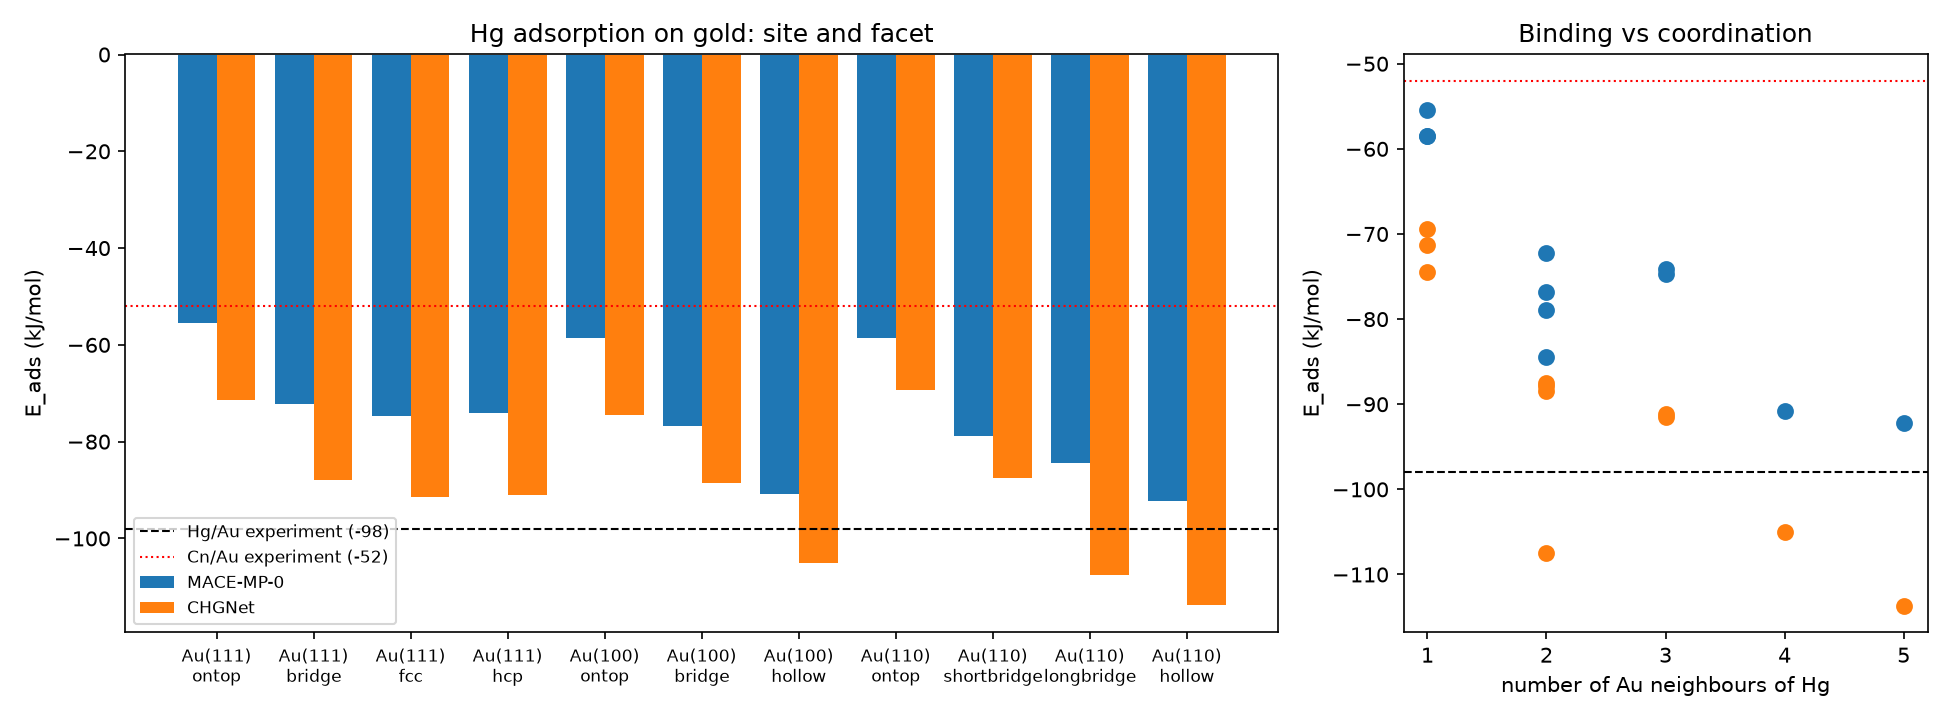
\includegraphics[width=\textwidth]{figures/Eads_facets.png}
\caption{Hg adsorption energies on 11 sites of three gold facets (left) and versus the number of Au atoms
in contact with Hg (right). Dashed: experimental Hg/Au~\cite{eichler2013}; dotted: Cn/Au~\cite{eichler2007}.}
\label{fig:eads}\end{figure}

\begin{table}[h]\centering
\caption{Adsorption energies (kJ/mol) and number of nearest Au neighbours $n$.}\label{tab:sites}
\begin{tabular}{llcrr}\toprule
Facet & Site & $n$ & MACE-MP-0 & CHGNet\\\midrule
Au(111) & ontop & 1 & $-55.4$ & $-71.3$\\
        & bridge & 2 & $-72.2$ & $-87.9$\\
        & fcc & 3 & $\mathbf{-74.7}$ & $\mathbf{-91.5}$\\
        & hcp & 3 & $-74.1$ & $-91.1$\\\midrule
Au(100) & ontop & 1 & $-58.5$ & $-74.5$\\
        & bridge & 2 & $-76.8$ & $-88.5$\\
        & hollow & 4 & $\mathbf{-90.8}$ & $\mathbf{-105.0}$\\\midrule
Au(110) & ontop & 1 & $-58.5$ & $-69.4$\\
        & short bridge & 2 & $-78.9$ & $-87.5$\\
        & long bridge & 2 & $-84.5$ & $-107.4$\\
        & hollow & 5 & $\mathbf{-92.2}$ & $\mathbf{-113.7}$\\\midrule
\multicolumn{3}{l}{Experiment, Hg/Au~\cite{eichler2013}} & \multicolumn{2}{c}{$\approx-98$}\\\bottomrule
\end{tabular}\end{table}

\paragraph{Site preference.} Both potentials give the same ranking on every facet: ontop $<$ bridge $<$
hollow. Binding grows with the number of Au neighbours (Fig.~\ref{fig:eads}, right), as expected for a
closed-shell atom bound mainly by polarisation and dispersion-like interactions. On Au(111) the fcc and hcp
hollows are degenerate within \SI{0.6}{kJ/mol}.

\paragraph{Facet dependence.} The close-packed Au(111) binds Hg most weakly; the more open Au(100) and Au(110)
bind it 14--22\,kJ/mol more strongly. For thermochromatography this means that a polycrystalline or rough
gold detector will retain Hg more strongly than an ideal (111) surface.

\paragraph{Model dependence.} The two MLIPs differ systematically by 9--23\,kJ/mol, CHGNet always binding more
strongly. This spread is as large as the facet effect, so the choice of potential is itself a major source of
uncertainty. Compared with the experimental $\approx98$\,kJ/mol, MACE-MP-0 underbinds on every site, while
CHGNet brackets the experiment: $-91.5$\,kJ/mol on Au(111) and $-105$ to $-114$\,kJ/mol on the open facets.
Both models clearly reproduce that Hg binds to gold much more strongly than Cn (52\,kJ/mol).

\section{Convergence and lattice-strain tests}
\begin{table}[h]\centering
\caption{Convergence of $E_\mathrm{ads}$ (kJ/mol) for Hg on the Au(111) fcc site. Default: 4 layers,
$3\times3$, \SI{12}{\AA} vacuum, model lattice constant.}\label{tab:conv}
\small\begin{tabular}{llrr}\toprule
Test & Value & MACE-MP-0 & CHGNet\\\midrule
Layers & 3 / 4 / 5 / 6 & $-74.5$ / $-74.7$ / $-74.8$ / $-74.7$ & $-91.0$ / $-91.5$ / $-91.1$ / $-91.0$\\
Cell & $2\times2$ / $3\times3$ / $4\times4$ & $-73.6$ / $-74.7$ / $-75.1$ & $-85.9$ / $-91.5$ / $-92.4$\\
Vacuum (\AA) & 8 / 12 / 16 & $-74.7$ / $-74.7$ / $-74.7$ & $-91.5$ / $-91.5$ / $-91.4$\\
Lattice (\AA) & own / 4.08 & $-74.7$ / $-69.9$ & $-91.5$ / $-86.5$\\\bottomrule
\end{tabular}\end{table}

Slab thickness and vacuum change $E_\mathrm{ads}$ by less than \SI{0.5}{kJ/mol}. The $2\times2$ cell is too
small for CHGNet (lateral Hg--Hg interaction through the periodic images), while going from $3\times3$ to
$4\times4$ changes the result by $\le\SI{0.9}{kJ/mol}$, so the production set-up is converged. Using the
experimental lattice constant instead of the model's own weakens binding by \SI{5}{kJ/mol} in both models;
together with the restriction to the bridge site, this explains why the baseline MACE script gives $-0.727$\,eV
instead of $-0.774$\,eV.

\section{Discussion and limitations}
\begin{itemize}
\item MACE-MP-0 and CHGNet are trained on PBE data from the Materials Project, which contain few
adsorbate-on-surface configurations and no explicit dispersion correction; PBE itself is known to underbind
closed-shell adsorbates. The good agreement of CHGNet with experiment may partly be fortuitous.
\item Relativistic effects enter only implicitly, through the scalar-relativistic PBE training data.
Spin--orbit coupling, which is decisive for Cn, is absent, so these potentials cannot be transferred to Cn
without new relativistic training data.
\item $E_\mathrm{ads}$ is a static \SI{0}{K} energy; the experimental quantity is an enthalpy derived from a
deposition temperature, and the detector surface is not an ideal single crystal.
\end{itemize}

\section{Conclusions and outlook}
A complete Linux/ASE workflow for Hg on gold was built from the baseline scripts: 11 sites on three facets, two
universal MLIPs, and convergence checks, each run in a few minutes on a laptop CPU. The physical trends
(hollow sites, open facets, coordination dependence) are robust across models, while the absolute binding
energy depends on the potential by up to \SI{23}{kJ/mol}. Natural next steps are: (i) adding D3 dispersion and
newer foundation models (MACE-MPA-0, MACE-OMAT-0, SevenNet); (ii) a small set of relativistic DFT reference points
for Hg/Au to fine-tune an MLIP; (iii) stepped and reconstructed surfaces such as Au(110)-(1$\times$2); and (iv)
the same workflow for Cn once relativistic reference data are available.

\paragraph{Code and data.} Scripts (\texttt{production.py}, \texttt{convergence.py}, \texttt{plot.py}), CSV
results and structures are available at \url{https://github.com/aszad-akib/hg-on-gold-mlip}.

\begin{thebibliography}{9}
\bibitem{eichler2007} R.~Eichler \emph{et al.}, ``Chemical characterization of element 112'', \emph{Nature}
\textbf{447}, 72 (2007).
\bibitem{eichler2013} R.~Eichler, ``First foot prints of chemistry on the shore of the Island of Superheavy
Elements'', \emph{J.\ Phys.: Conf.\ Ser.}\ \textbf{420}, 012003 (2013), arXiv:1212.4292.
\bibitem{ase} A.~H.~Larsen \emph{et al.}, ``The atomic simulation environment'', \emph{J.\ Phys.: Condens.\
Matter} \textbf{29}, 273002 (2017).
\bibitem{mace} I.~Batatia \emph{et al.}, ``A foundation model for atomistic materials chemistry'',
arXiv:2401.00096 (2023).
\bibitem{chgnet} B.~Deng \emph{et al.}, ``CHGNet as a pretrained universal neural network potential for
charge-informed atomistic modelling'', \emph{Nat.\ Mach.\ Intell.}\ \textbf{5}, 1031 (2023).
\bibitem{repo} M.~Ilia\v{s}, \texttt{open-collection}, \url{https://github.com/miroi/open-collection}.
\end{thebibliography}
\end{document}
